\documentclass[border=4pt]{standalone}
\usepackage{tikz}
\usetikzlibrary{arrows.meta,positioning,shapes.geometric}
\begin{document}
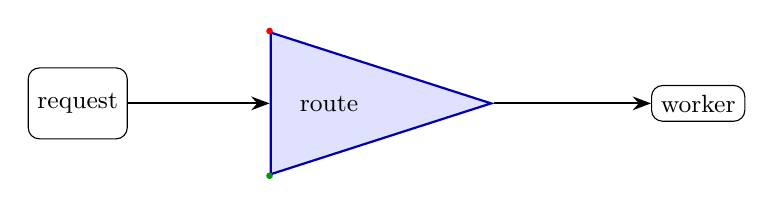
\begin{tikzpicture}[
  >=Stealth,
  node distance=18mm,
  every node/.style={font=\small},
  route/.style={
    isosceles triangle,
    isosceles triangle apex angle=54,
    isosceles triangle stretches,
    minimum width=18mm,
    minimum height=28mm,
    inner sep=2mm,
    draw=blue!70!black,
    fill=blue!12,
    thick
  }
]
  \node[draw,rounded corners,minimum height=9mm] (input) {request};
  \node[route,right=of input] (route) {route};
  \node[draw,rounded corners,right=20mm of route.apex] (output) {worker};
  \draw[->,thick] (input.east) -- (route.west);
  \draw[->,thick] (route.apex) -- (output.west);
  \fill[red] (route.left corner) circle (1.2pt);
  \fill[green!60!black] (route.right corner) circle (1.2pt);
\end{tikzpicture}
\end{document}
